\graphicspath{{fig/circ_stats_intro/}}

\chapter{Directional statistics}	
\label{cha:direct_stats}

%NOTES: consider adding section on circular distributions. Show limiting result of von Mise distribution as normal distribution

Circular data arises naturally in the study of collective behaviour. In particular, a researcher in the field will undoubtedly encounter data describing the direction of motion of individuals. Given any dataset, the first instinct of the practitioner is to summarise and visualise the data. However, such a researcher should proceed with caution --- circular data cannot be treated as if it were its linear counterpart.

In this short chapter we shall consider why standard techniques, methods and summaries are inappropriate to use with circular data. After this realisation, we proceed to introduce some useful techniques which can be used to handle and visualise directional data.

\section{Conventions}
\label{sec:conventions}

Directions can be represented as rotations with respect to some zero--direction, or origin. The practitioner is free to chose the zero--direction as they feel appropriate. In a similar way, the practitioner may choose whether a clockwise or anti--clockwise rotation is taken as the positive direction.

Recall that angles may be represented in units of degrees or radians. To convert between degrees and radians we may multiply by a factor of $\pi/180$\textdegree.

In this thesis we shall define the zero angle as the direction from $(0, 0)$ and along the positive $x$--axis. For the most part, we shall measure angles in units of radians, and take anti--clockwise rotations as the positive direction. The schematics of this setup are illustrated in \cref{subfig:radian_axes}. Occasionally, we shall appeal to degrees and their comparative intuitiveness, and in these cases we shall use the setup illustrated in  \cref{subfig:degree_axes}.

\begin{figure}
\centering
	\begin{subfigure}[b]{0.5\textwidth}
		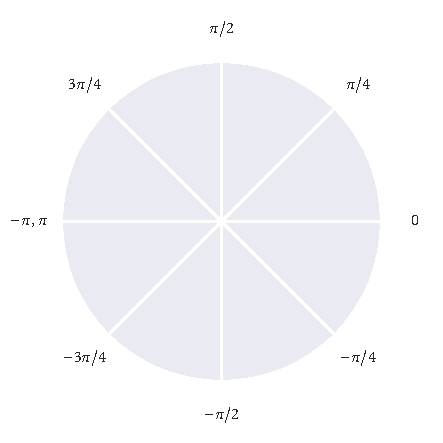
\includegraphics{radian_axes.pdf}
		\caption{}
		\label{subfig:radian_axes}
	\end{subfigure}%
	\begin{subfigure}[b]{0.5\textwidth}
		\centering
		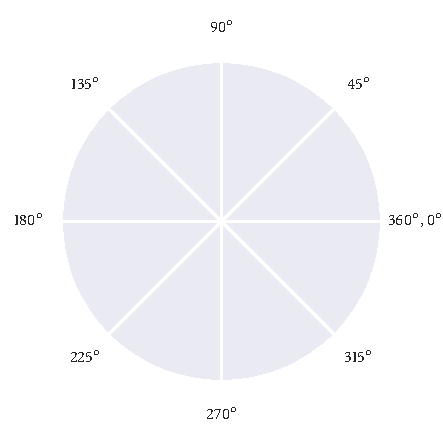
\includegraphics{degree_axes.pdf}
		\caption{}
		\label{subfig:degree_axes}
	\end{subfigure}
	\caption{Comparing \subref{subfig:radian_axes}: radian and \subref{subfig:degree_axes}: degree measuring conventions adopted in this thesis.}
	\label{fig:compare_axes}
\end{figure}

\section{Visualisation}
\label{sec:circular_visualisation}

In possession of a dataset, one of the first instincts of the scientist is to visualise their data. The researcher is undoubtedly familiar with a large number of graph types. Yet choosing the most suitable graph to display a given dataset is crucial in making an informative plot.

Traditional histograms are not very good for visualising directional data. Polar histograms (sometimes known as rose plots) make the visualisation of such data easier. Instead of using bars, as the histogram does, the rose plot bins data into sectors of a circle. The area of each sector is proportional to the frequency of data points in the corresponding bin.

\begin{figure}
	\begin{subfigure}[b]{0.48\textwidth}
		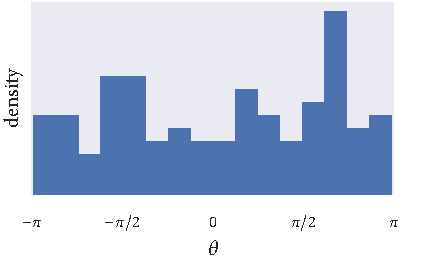
\includegraphics{unif_angle_hist.pdf}
		\caption{}
		\label{subfig:unif_angle_hist}
	\end{subfigure}%
	\hspace{0.01\textwidth}
	\begin{subfigure}[b]{0.48\textwidth}
		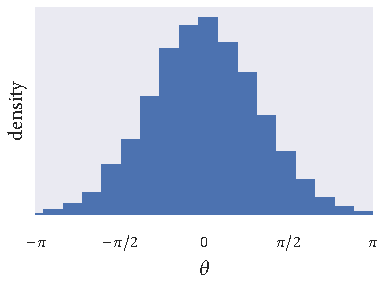
\includegraphics{norm_angle_hist.pdf}
		\caption{}
		\label{subfig:norm_angle_hist}
	\end{subfigure}
	\caption{Using histograms to visualise \subref{subfig:unif_angle_hist}: 100 samples from $U(-\pi, \pi)$ and \subref{subfig:norm_angle_hist}: 10\thinspace 000 draws from $N(0, 1)$.}
	\label{fig:angle_hist}
\end{figure}

\begin{figure}
	\begin{subfigure}[b]{0.45\textwidth}
		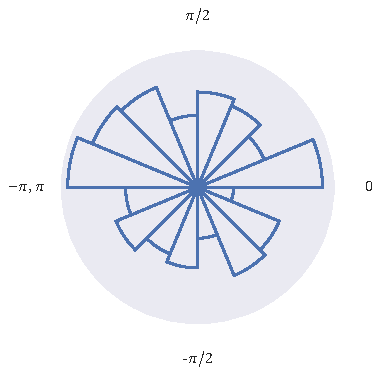
\includegraphics{unif_angle_rose.pdf}
		\caption{}
		\label{subfig:unif_angle_rose}
	\end{subfigure}%
	\hspace{0.05\textwidth}%
	\begin{subfigure}[b]{0.45\textwidth}
		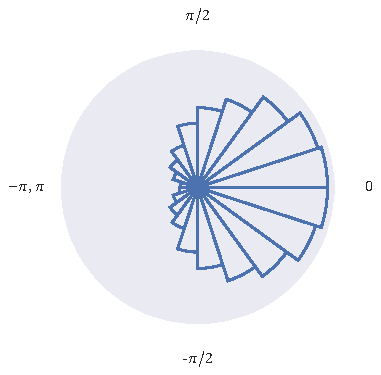
\includegraphics{norm_angle_rose.pdf}
		\caption{}
		\label{subfig:norm_angle_rose}
	\end{subfigure}
	\caption{Using polar histograms to visualise the dataset generated from \subref{subfig:unif_angle_rose}: $U(-\pi,\pi)$ and \subref{subfig:norm_angle_rose}: $N(0, 1)$.}
	\label{fig:angle_rose}
\end{figure}
To advocate the advantages of the rose plot we shall visualise two randomly generated datasets. The first dataset consists of 100 realisations from a uniform $U(-\pi,\pi)$ distribution, and the second dataset consists of 10\thinspace 000 draws from a normal $N(0, 1)$ distribution.

In \cref{fig:angle_hist} we visualise the two datasets using traditional histogram plots. From this figure we get a good idea of the distribution of the data, however we get no sense of direction. The traditional histogram leaves us to interpret the directions ourselves.

In \cref{fig:angle_rose} we visualise the same data as before. Here we also get a good idea of how the directions are distributed. However, using the rose plot means we get a very intuitive representation of direction. We therefore consider the rose plot a very useful method of displaying circular data which is easy to interpret.

\section{Summary statistics}
\label{sec:summary_stats}

Summary statistics are a useful tool to give an idea of the general characteristics of a dataset. Probably the first statistic which we learn to compute is the arithmetic mean. The arithmetic mean, however, is not an appropriate measure to use with circular data.

Consider that we wish to take an average of the angles $10$\textdegree and $350$\textdegree. Using the arithmetic mean we compute an average of $180$\textdegree --- however, this average points in the opposite direction to which we intuitively expect. In \cref{subfig:arith_mean} we visualise this surprising result.

\begin{figure}
	\begin{subfigure}[b]{0.45\textwidth}
		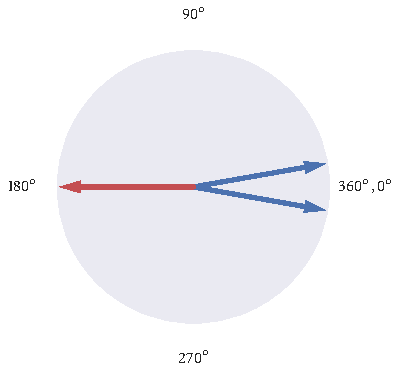
\includegraphics{arith_mean.pdf}
		\caption{Arithmetic mean (red).}
		\label{subfig:arith_mean}
	\end{subfigure}%
	\hspace{0.05\textwidth}
	\begin{subfigure}[b]{0.45\textwidth}
		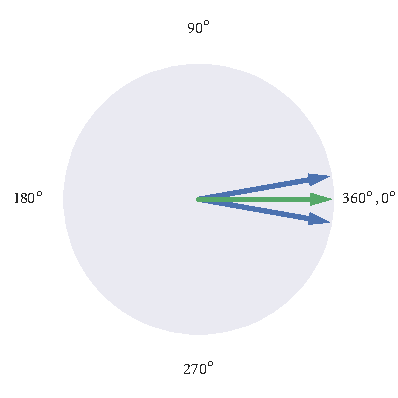
\includegraphics{circ_mean.pdf}
		\caption{Circular mean (green).}
		\label{subfig:circ_mean}
	\end{subfigure}
	\caption{Computing the average of two angles with two different means. The blue arrows ($10$\textdegree and $350$\textdegree) represent the directions to be averaged and the green and red arrows show the average computed by the method.}
	\label{fig:visualise_mean}
\end{figure}

Before introducing the circular mean it is first necessary to introduce the $\atantwo$ function. The $\atantwo$ function dates back to the Fortran programming language \parencite{organick66}. It was introduced to overcome some of the inconveniences inherent in the $\atan$ (or $\tan^{-1}$) function. For starters, the inverse tangent function has codomain $(-\pi/2, \pi/2)$, though we are often interested in directions in the range $(-\pi, \pi]$. In addition to this, the $\arctan$ function is not quadrant--aware --- it cannot distinguish between opposite directions (directions which differ by $\pi$ radians). As an example, consider calculating the direction from the $x$--axis to the ray extending from the origin to $(1, 1)$. Naturally, we'd reach for $\tan^{-1}$ to compute the angle as $\tan^{-1}(1/1) = \pi/4$, as expected. Now, consider that we wish to calculate the direction from the $x$--axis to the ray extending from $(0, 0)$ to $(-1, -1)$. By inspection, or intuitively, we expect an answer of $-3\pi/4$ --- however, we compute the answer as $\tan^{-1}(-1/-1) = \pi/4$. The angle calculated using the inverse tangent function points in the opposite direction to what we expect.

\begin{figure}
	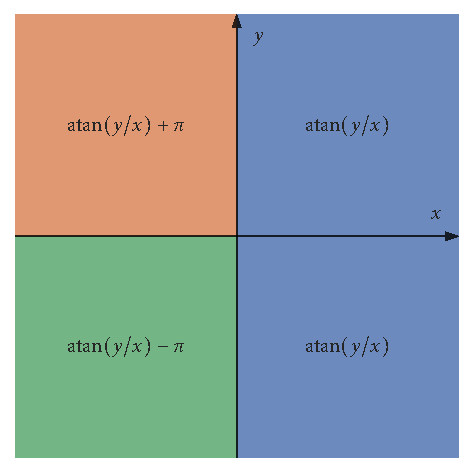
\includegraphics{atan_quadrants.pdf}
	\caption{An illustration of the quadrant corrections made by $\atantwo$.}
	\label{fig:atan_quadrants}
\end{figure}

The $\atantwo$ function, however, does not have these shortcomings. The function is constructed to be quadrant--aware: correcting the computations of $\tan^{-1}$ to return the directions we intuitively expect. It does this by adding a correction term that depends on which quadrant contains the point $(x, y)$. The handling of the four quadrants by $\atantwo$ is visualised in \cref{fig:atan_quadrants}. With these considerations, $\atantwo$ can be realised as:

\begin{equation}
\label{eq:atantwo}
	\atantwo(y, x) = 
	\begin{cases}
		\atan(y/x) & \text{ if } x > 0, \\
		\atan(y/x) + \pi & \text{ if } x < 0 \text{ and } y \geq 0, \\
		\atan(y/x) - \pi & \text{ if } x < 0 \text{ and } y < 0, \\
		\pi/2  & \text{ if } x = 0 \text{ and } y > 0, \\
		- \pi/2 & \text{ if } x = 0 \text{ and } y < 0, \\
		\text{undefined} & \text{ if } x = 0 \text{ and } y = 0. \\
	\end{cases}
\end{equation}

When averaging a set of angles we must not use the arithmetic mean. Instead, we must refer to the circular mean. Given a set of angles $\bm{\theta} = (\theta_1, \ldots, \theta_n)^T$, we may compute their circular mean as:
\begin{equation}
	\label{eq:circ_mean}
	\langle \bm{\theta} \rangle = \atantwo\bigg(\frac{1}{n} \sum_{j=1}^n \sin(\theta_j), \frac{1}{n} \sum_{j=1}^n \cos(\theta_j)\bigg),
\end{equation}
where the $\atantwo$ function is defined in \cref{eq:atantwo}.

The definition of the circular mean given in equation \cref{eq:circ_mean} works by converting the angles into Cartesian co--ordinates --- representing the directions as points on the unit circle. The centre of mass of the Cartesian co--ordinates is then computed, and the resulting position is converted back to a direction, resulting in our mean angle.
